\section{Marco Teorico}

    \subsection{Revisión de la literatura}
        El humano tiene una forma de aprendizaje muy particular, la cual se basa del estudio, donde lee, escribe y practica acerca de
        su tema de interes, pero dicho aprendizaje se puede ir olvidando, esto es una acción muy común que a cualquier persona.
        Existen estudios donde se comenta que existen tres motivos del porque se olvidan las cosas, proviene parte de la regularización de las emociones,
        el como se adquirierón los conocimientos y porque el olvido es un proceso por el cual el ser humano transita a lo largo de su vida \cite{Nrby2015}. Pero cabe
        mencionar que esto no es lo único que causa la perdida de memoria, ya que existe la déficits de memoria. 

    \subsection{Aprendizaje Humano}
        Al momento de hablar del aprendizaje humano, se debe de hablar de la ciencia cognitiva, que es quien se encarga de descubrir esta incognita,
        esta cienca lo estudia de un modo multidisiplinario, el cual abarca las \'areas de \cite{bransford2000}: 
        \begin{itemize}
            \item La antropología.
            \item La lingüística.
            \item La filosofía.
            \item La sicología del desarrollo.
            \item La ciencia de la computación. 
            \item La neurociencia.
        \end{itemize}
        Con el metodo de esta cienca podemos descubrir dos tipos de aprendizaje que son:
        \begin{enumerate}
            \item Aprendizaje con Compresi\'on.
            \item Aprendizaje Activo.
        \end{enumerate}
        \subsubsection{Aprendizaje con Compresi\'on}
            La comprensi\'on es una activiadad la cual se ha generado al momento de realizar cualquier tipo de lectura.\\
            Al hablar de este tema nos enfocamos en el \'ambito estudiantil que es donde m\'as se maneja esta t\'actica, esto es una
            practica algo compleja, sist\'ematica y organizada, ya que nos da el significado de la literatura, gracias a esto se puede
            obtener el contexto de la literatura.

            Al conocer esto podemos decir con seguridad que para cualquier tipo de aprendizaje la comprensi\'on es 
            una parte primordial \cite{perez2014}.

        \subsubsection{Aprendizaje Activo}
            El aprendizaje de la forma en la que la conocemos no es del todo efectiva, se dice esto porque parte del sistema de educaci\'on porque la manera 
            correcta es con el principio de \textit{belongingness} el cual esta asociado al estimulo con su respuesta
            y esto es lo m\'as importante para que el ser humano pueda aprender cualquier cosa.\\
            Este tipo de aprendizaje se basa en la recepci\'on de conocimientos y la pr\'actica donde se ponen en marcha los conocimientos adquiridos.\\
            Otro concepto importante aqu\'i es la tautolog\'ia doble (\textit{selbstt\"atiges Lernen}) que en palabras informales es convertirse en autodidacta, 
            podemos observar que esto pertener a dicho de aprendizaje porque usa el principio mencionado anteriormente \cite{Huber2008}.



    \subsection{Aprendizaje Incremental}
        Con el pasar de los años la tecnología a evolucionado, eso quiere decir que el Aprendizaje Automático se ha actualizado, que la 
        cantidad de datos va aumentado con más frecuencia.
        
        Lo podemos verificar como \textit{"Una tarea de aprendizaje es incremental si los ejemplos de entrenamiento usados para 
        resolverla están disponibles en horas extras, generalmente uno a la vez"} \cite{GiraudCarrier2000}, si los resultados no se 
        necesitan de manera urgente, este tipo de trabajos serán resueltos por algoritmos de aprendizaje no incremental. 

        Una área donde esto es de mucha utilidad es la \textit{Robotica} porque este necesitan estar en constante entrenamiento \cite{GiraudCarrier2000}.

        Dicha forma de aprender fue inspirada en la forma que el humano aprende y esta es una forma más rápida, fue por esto que fue adoptada 
        por el aprendizaje maquina.

        Con el paso del tiempo se ha convertido en un paradigma del aprendizaje autómatico, aqui el aprendizaje toma el lugar de nuevos ejemplos para juntarlos 
        y conforme van aprendiendo estos toman el lugar de los ejemplos ya aprendidos \cite{liu2015}.

        \subsubsection{Algoritmos de Aprendizaje Incremental}
            \textit{"Un algoritmo de aprendizaje es incremental si,
            para cualquier muestra de entrenamiento dada:
            \begin{equation}
                e_{1} , .... , e_{s}
			\end{equation}
            , produce un secuencia de hipótesis 
            \begin{equation}
                h_{0} , h_{1}, . . . , h_{n} 
            \end{equation}
            , tal que hi+1 depende solo de hola y del ejemplo actual e"} \cite{GiraudCarrier2000}, como 
            observamos estos son algoritmos que permiten a la inteligencia artificial poder realizar actividades de predicci\'on 
            de una manera m\'as eficaz.\\
            Un ejemplo del uso de esta rama esta el proyecto \textit{COBWEB} donde se trata de categorizar el n\'umero de cluster y la pertenencia 
            de dichas categor\'ias por medio de una m\'etrica probabil\'istica global, esto lo realiza por medio de que se agrega 
            una nueva categor\'ia, este proceso lo que realizara es actualizar todas las probabilisticas con los nuevos datos recabados \cite{fisher1987}.
    
    \subsection{Redes Neuronales Artificiales}
        
        Las redes neuronales artificiales (RNA) son procesos los cuales contienen simples unidades de procesamientos. \\
        Como podemos darnos cuenta, al mencionar RNA lo primero que se nos viene a la mente es el procesamiento biol\'ogico por el que transita el 
        cerebro humano. El m\'etodo principal de las redes neuronales es sacarle el maximo poder a los algoritmos de aprendizaje maquina, ya que las redes neuronales 
        tiene un antecedente biol\'ogico.

        Tiene demasiadas utilidades las cuales ayudan a distintas problematicas, algunas de las funciones que tiene son \cite{liu2015}:

        \begin{enumerate}
            \item No linealidad.
            \item Mapeo entrada-salida.
            \item Aprendizaje robusto a errores en los datos de entrenamiento. 
            \item Entre otros.
        \end{enumerate}

        Existen varios tipos de Redes Neuronales tales como: 
        \begin{itemize}
            \item Redes Neuronales de Perceptr\'on Multicapa.
            \item Redes Neuronales Convolucionales.
            \item Entre otras.
        \end{itemize}
    
        \subsubsection{Redes Neuronales de Perceptr\'on Multicapa}

            Al momento de mapear el progreso de una red nos sirve para conocer buscar un camino adecuado entre la capa de entrada y salida, esto se puede hacer 
            con problemas de una sola neurona, pero no se puede n resolver problemas no lineales, es aqu\'i donde entran los perceptrones
            multicapas, los cuales rompen con esta limitaci\'on.

            Estas neuronas est\'an compuestas de 3 capas:
            \begin{enumerate}
                \item Capas de entrada.
                \item Capas ocultas.
                \item Capas de salida.
            \end{enumerate}

            Los datos de entrada se van a ir propagando capa por capa, hasta llegar a la capa final, donde ya paso
            por una funci\'on de activaci\'on donde se rompio la no linealinidad, para poder llegar a un resultado \cite{liu2015}.

            \begin{figure}[H]
                \centering
                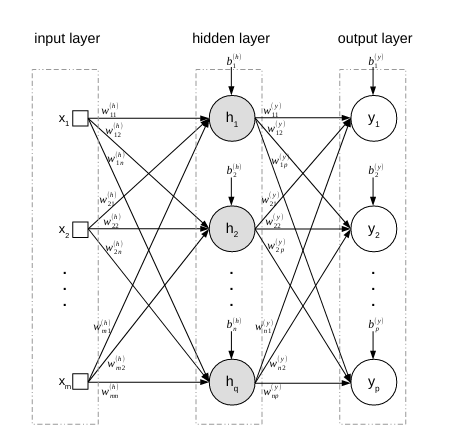
\includegraphics[width=\columnwidth]{MLP.png}
                \caption{Red Neuronal de Perceptr\'on Multicapa \cite{liu2015}}
                \label{fig:fig1}
            \end{figure}

        \subsubsection{Redes Neuronales Convolucionales}

            Este tipo de red trabaja con el uso de imagenes, por lo general se suele trabajar con imagenes de alta calidad, el \'unico poroblema que se tiene 
            al momento de que sean de alta resoluciones son:
            \begin{itemize}
                \item El tiempo de entrenamiento sea enorme.
                \item El tiempo de testo sea muy tardio.
            \end{itemize}

            Consta de diversas multicapas alternadas, al final tiene una red perceptron multicapa.
            La entrada de una red convolucional, con diferentes medidas en altura y ancuhura de imagen, para el uso 
            de los proyectos se trabajan en escalas de grises, las cuales contienen filtros y cada filtro tiene distintos 
            rasgos y caracteristicas de tamaño. Cada capa es submustreo de m\'inimo a m\'aximo muestre, donde se toman valores 
            desde 2 im\'agenes pequeñas hasta no mas de 5 im\'agenes grandes.

            Antes o despu\'es del submuestreo se aplica la activaci\'on sigmoidal para cada mapeo de rasgos \cite{duran2017}.

            \begin{figure}[H]
                \centering
                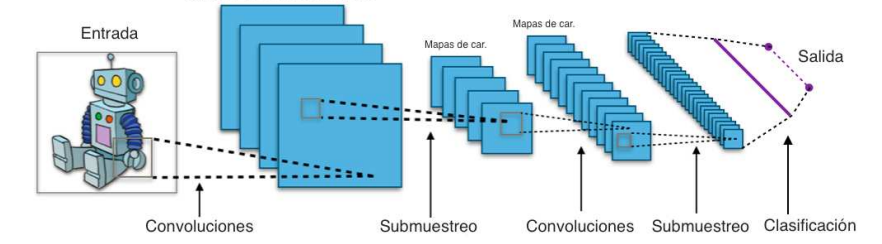
\includegraphics[width=\columnwidth]{esquemaRedConvolucional.png}
                \caption{Esquema de una Red Convolucional \cite{duran2017}}
                \label{fig:fig2}
            \end{figure}